% Opcje klasy 'iithesis' opisane sa w komentarzach w pliku klasy. Za ich pomoca
% ustawia sie przede wszystkim jezyk oraz rodzaj (lic/inz/mgr) pracy.
\documentclass[shortabstract]{iithesis}

\usepackage[utf8]{inputenc}
\usepackage{amsthm}
\usepackage{graphicx}
\usepackage{float}
\usepackage{xurl}

%%%%% DANE DO STRONY TYTUŁOWEJ
% Niezaleznie od jezyka pracy wybranego w opcjach klasy, tytul i streszczenie
% pracy nalezy podac zarowno w jezyku polskim, jak i angielskim.
% Pamietaj o madrym (zgodnym z logicznym rozbiorem zdania oraz estetyka) recznym
% zlamaniu wierszy w temacie pracy, zwlaszcza tego w jezyku pracy. Uzyj do tego
% polecenia \fmlinebreak.
% \polishtitle    {Implementacja aplikacji magazynu sprzętu \fmlinebreak elektronicznego z wykorzystaniem\fmlinebreak Domain Driven Design}
\polishtitle    {Implementacja aplikacji webowej służącej \fmlinebreak do obsługi turniejów do gry \fmlinebreak Counter Strike: Global Offensive}
\englishtitle   {Implementation of web application \fmlinebreak used to organize tournaments for \fmlinebreak Counter Strike: Global Offensive}
\polishabstract{Z roku na rok rośnie liczba organizowanych profesjonalnych turniejów w wielu grach, jednak narzędzia wspomagające organizację turniejów są zwykle niedostępne dla widzów. Implementacja tej aplikacji miałaby się przyczynić do ułatwienia organizacji turniejów dla każdego. Z założenia miałaby głównie wspierać:

\begin{itemize}
    \item system ligowy, pucharowy i mieszany,
    \item rozgrywane mecze w formacie BO1/3/5 (Best of...),
    \item odrzucanie map przez kapitanów obu drużyn,
    \item możliwość tworzenia turniejów prywatnych i publicznych,
    \item panel administracyjny do zarządzania rozgrywkami.
\end{itemize}

Ponadto implementacja będzie korzystać z dwóch frameworków front-endowych: Vue oraz Cycle.js, które prezentują całkowicie odmienne podejście do programowania aplikacji webowych.}
\englishabstract{The number of organized professional tournaments in many games is growing every year, but the tools for organizing tournaments are usually inaccessible to spectators. Implementation of this application would contribute to enabling the organization of tournaments for everyone. By design it would mainly support:

\begin{itemize}
    \item league, cup and mixed system,
    \item matches played in BO1/3/5 (Best of...) format,
    \item discarding of maps by the captains of both teams,
    \item possibility to create private and public tournaments,
    \item administration panel to manage the games.
\end{itemize}

Moreover, the implementation will use two front-end frameworks, i.e. Vue.js and Cycle.js, which present a completely different approach to web application programming.
}
% w pracach wielu autorow nazwiska mozna oddzielic poleceniem \and
\author         {Tomasz Woszczyński}
% w przypadku kilku promotorow, lub koniecznosci podania ich afiliacji, linie
% w ponizszym poleceniu mozna zlamac poleceniem \fmlinebreak
\advisor        {dr Wiktor Zychla}
%\date          {}                     % Data zlozenia pracy
% Dane do oswiadczenia o autorskim wykonaniu
%\transcriptnum {}                     % Numer indeksu
%\advisorgen    {dr. Jana Kowalskiego} % Nazwisko promotora w dopelniaczu
%%%%%

%%%%% WLASNE DODATKOWE PAKIETY
%
% \usepackage{graphicx,listings,amsmath,amssymb,amsthm,amsfonts,tikz}
%
%%%%% WŁASNE DEFINICJE I POLECENIA
%
\theoremstyle{definition} \newtheorem{definition}{Definicja}[]
\theoremstyle{remark} \newtheorem{remark}[definition]{Observation}
\theoremstyle{plain} \newtheorem{theorem}[definition]{Theorem}
\theoremstyle{plain} \newtheorem{lemma}[definition]{Lemma}
\renewcommand \qedsymbol {\ensuremath{\square}}
% ...
%%%%%

\begin{document}

%%%%% POCZĄTEK ZASADNICZEGO TEKSTU PRACY

\chapter{Wprowadzenie}
\section{Motywacja}
W ciągu ostatnich lat brałem udział w kilkunastu amatorskich, jak i półprofesjonalnych turniejach offline w grze Counter Strike: Global Offensive i niejednokrotnie byłem świadkiem chaosu, który powstawał poprzez niepoprawne podejście organizatorów do organizacji zawodów. Zwykle wiązało się to z prowadzeniem wszelkich statystyk w niepoprawnie przygotowanych arkuszach kalkulacyjnych, albo co gorsza - na kartkach, bez żadnych narzędzi wspomagających automatyzację procesu. Kolejnym sporym problemem było wybieranie i odrzucanie map przez obie drużyny, zwykle gracze musieli chodzić po ogromych salach i się szukać, a informacje o wybranych mapach przekazywali administratorom po kilku minutach. Stworzenie aplikacji do organizacji turniejów było pomysłem, który miał wyjść na przeciw oczekiwaniom i zarówno ułatwić udział w turniejach, jak i ich organizację.

\section{Opis aplikacji CStrikers}
Aplikacja CStrikers sprawia, że organizatorzy mogą w łatwy sposób tworzyć turnieje różnych rodzajów, a gracze brać w nich udział. Najczęściej spotykanymi rodzajami turniejów są system pucharowy, system ligowy oraz system mieszany. Wszystkie mecze rozgrywane w turnieju są rozgrywane w jednym z systemów: Best Of 1, Best Of 3 albo Best of 5. Rozgrywane mecze są na mapach wybieranych przez obie drużyny - ich wybór odbywa się na żywo poprzez odrzucanie i wybieranie map przez kapitanów obu drużyn. Po każdym meczu uzupełniane są statystyki końcowe każdej z map, a następnie na ich podstawie wyznaczany jest wynik końcowy.


\section{Ważniejsze pojęcia i skróty}
\begin{definition}
    Counter Strike: Global Offensive --- gra z gatunku first-person shooter stworzona przez Valve w 2012. roku. Do każdej rozgrywki przystępują dwie drużyny, każda z nich składa się z 5 graczy biorących aktywnie udział (często spotyka się zmienników, jednak w jednym momencie może grać tylko 5 osób). Celem każdej z drużyn jest wygranie 16 rund, lub więcej w przypadku dogrywki. W kolejnych rozdziałach tytuł gry skracany będzie do CSGO.
\end{definition}

\begin{definition}
    System pucharowy --- sposób rozgrywania turnieju polegający na rozgrywaniu bezpośrednich pojedynków. Zwycięzca spotkania przechodzi do kolejnej rundy, a pokonany odpada z turnieju. W turnieju może wziąć udział liczba drużyn będąca potęgą liczby 2. Często spotykanymi określeniami są Single Elimination oraz Knock-out.
\end{definition}

\begin{definition}
    System ligowy --- sposób rozgrywania turnieju, w którym każda drużyna gra ze wszystkimi pozostałymi. Wyniki końcowe ligi są obliczane na podstawie wygranych meczów, a w przypadku takiej samej liczby wygranych brane są pod uwagę również wygrane i przegrane rundy. Innymi określeniami na system ligowy są również system kołowy, każdy z każdym oraz round-robin.
\end{definition}

\begin{definition}
    System mieszany --- sposób rozgrywania turnieju będący połączeniem systemu ligowego oraz systemu pucharowego. Uczestnicy turnieju są rozdzielani do czterodrużynowych grup, w których rozgrywa się mecze w systemie kołowym, a następnie dwie najlepsze drużyny z każdej grupy przechodzą do kolejnego etapu rozgrywanego w systemie pucharowym.
\end{definition}

\begin{definition}
    Best of $N$ --- określenie na typ pojedynczego meczu. $N$ oznacza liczbę maksymalnie rozgrywanych map w bezpośrednim starciu, z czego aby wygrać cały mecz, należy wygrać $\left\lceil \frac{N}{2} \right\rceil$ map. W systemie BO1 kapitanowie odrzucają mapy dopóki nie zostanie ostatnia, na której będzie odbywał się mecz. Wybór rozgrywanych map w systemie BO3 odbywa się następująco: $B - B - P - P - B - B - P$, gdzie $B$ oznacza mapę zbanowaną (odrzuconą), a $P$ mapę wybraną. W systemie BO5 kapitanowie odrzucają po jednej mapie, a następnie wybierają kolejność rozgrywek na pozostałych mapach.
\end{definition}

\begin{definition}
    Framework --- szkielet definujący strukturę aplikacji oraz sposób jej działania. Projekt CStrikers wykorzystuje dwa frameworki front-endowe: Vue.js oraz Cycle.js.
\end{definition}

\chapter{Opis wykorzystanych frameworków}
\section{Vue.js}
Vue.js to framework napisany w języku JavaScript. Korzysta z architektury \textit{Model-View-ViewModel}. Powstał on w celu stworzenia bardziej elastycznego narzędzia niż istniejące dotychczas frameworki React.js oraz Angular. Vue charakteryzuje bardzo niski próg wejścia (m.in. dzięki bardzo dobrej dokumentacji), bardzo przejrzysta struktura kodu oraz cechuje go intuicyjność. Głównymi funkcjonalnościami wyróżniającymi ten framework są:
\begin{itemize}
    \item \textit{declarative binding}, czyli rozszerzenie standardu HTML o składnię wzorców, umożliwiające opisywać wyjście HTML na podstawie stanu JavaScript.
    \item \textit{reactivity} (reaktywność), czyli automatyczne śledzenie stanu JavaScript na podstawie zmian i aktualizowanie DOM.
\end{itemize}

Kolejnym dużym plusem jest zastosowanie \textit{Single-File Components}, a więc komponentów zawierających się w jednym pliku \texttt{*.vue}. SFC pozwala na enkapsulację logiki komponetentu w JavaScript, wzorca strony w HTML oraz styli CSS w jednym pliku. Podejście do programowania SFC jest zalecane przez autorów frameworku.

Nie jest to jednak jedyna możliwość implementowania aplikacji we Vue.js. Drugim sposobem jest podzielenie komponentu na kilka plików (JS, HTML oraz CSS) i połączenie ich wszystkich poprzez wywołanie metody \texttt{createApp} z modułu \texttt{vue}, a następnie zamontowania jej do wybranego ID z pliku HTML. To podejście jest jednak używane znacznie rzadziej, jako że przenaszalność komponentów znacząco maleje, co sprawia, że w aplikacji mógłby powstać bardzo powtarzalny kod.

\begin{figure}[H]
	\centering
	$\vcenter{\hbox{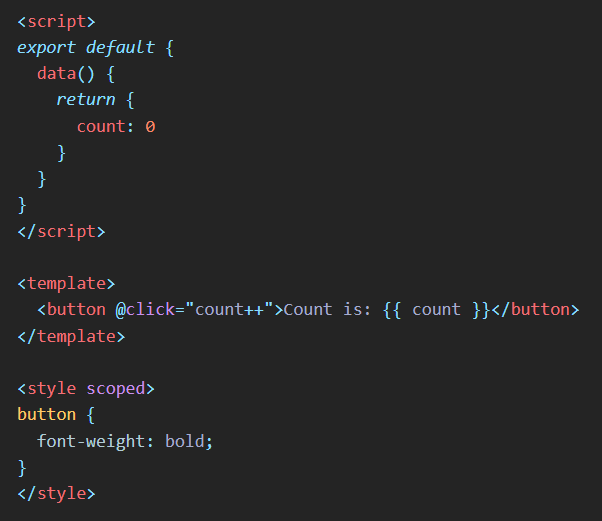
\includegraphics[width=0.8\textwidth]{images/vue-sfc-example.png}}}$
    \caption[]{Przykład prostego komponentu SFC \cite{bib:sfc}}
    \label{fig:vue-sfc}
\end{figure}

\begin{figure}[H]
	\centering
	$\vcenter{\hbox{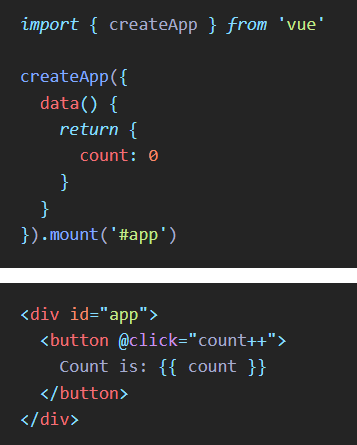
\includegraphics[width=0.65\textwidth]{images/vue-splitted-component.png}}}$
    \caption[]{Analogiczny komponent podzielony na pliki JS oraz HTML \cite{bib:vue-sfc}}
    \label{fig:vue-splitted}
\end{figure}

Ważną częścią Vue.js jest cykl życia komponentów. Każda instancja komponentu przechodzi przez serię kroków inicializacyjnych przy stworzeniu, a sam framework udostępnia możliwość dodania kodu do istniejących \textit{lifecycle hooks}. Dzięki temu programista może w łatwy sposób wpłynąć na działanie komponentu, wywołując w odpowiednich momentach zawołania API do bazy danych, inicializując wartości domyślne danych komponentów i inne.

\begin{figure}[H]
	\centering
	$\vcenter{\hbox{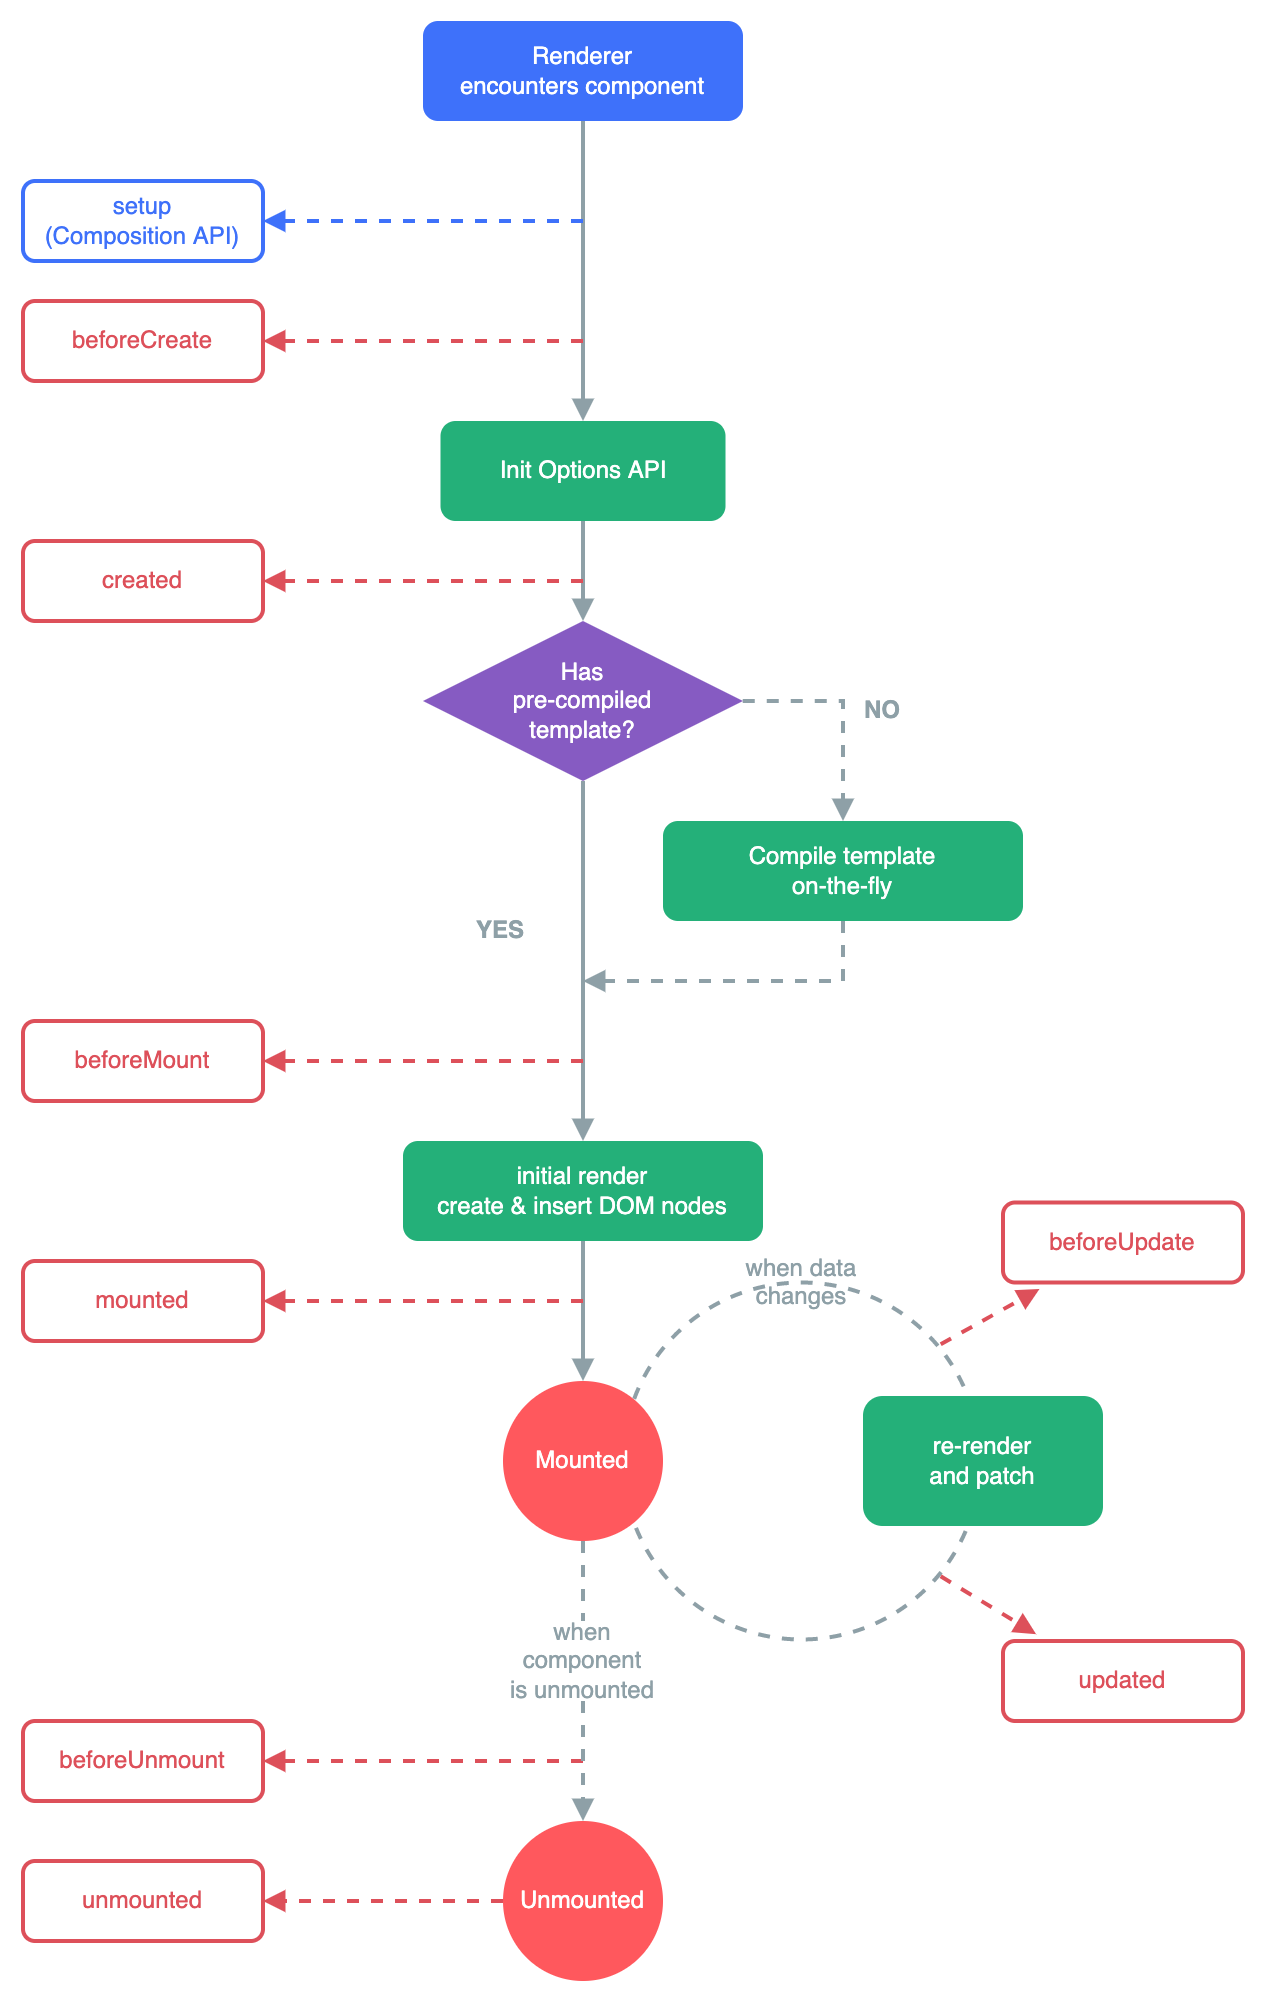
\includegraphics[width=0.8\textwidth]{images/vue-lifecycle.png}}}$
    \caption[]{Cykl życia komponentu Vue.js wraz z \textit{lifecycle hooks} \cite{bib:vue-lifecycle-hooks}}
    \label{fig:vue-lifecycle-hooks}
\end{figure}

\section{Cycle.js}
Cycle.js to funkcyjny i reaktywny framework JavaScript. Funkcyjność sprawia, że kod jest bardziej przewidywalny, a reaktywność pozwala na rozdzielenie kodu. Aplikacje Cycle.js są w pełni stworzone z funkcji, dzięki czemu na podstawie wejścia (argumentów funkcji) jest generowane przewidywalne wyjście, bez niepożądanych efektów I/O.

Elementem składowym są reaktywne strumienie z bibliotek takich jak \texttt{xstream}, \texttt{RxJS}, czy \texttt{Most.js}. Strukturyzacja aplikacji Cycle.js za pomocą strumieni usuwa problemy dotyczące zmian z zewnątrz, jako że wszystkie zmiany danych są wewnątrz strumieni. Strumień w \texttt{xstream} jest ciągiem wydarzeń, którym może wyemitować zero lub więcej wydarzeń oraz może się skończyć lub nie skończyć. Zakończenie się strumienia oznacza wykonanie jakiegoś działania lub wyemitowanie błędu.

\begin{figure}[H]
	\centering
	$\vcenter{\hbox{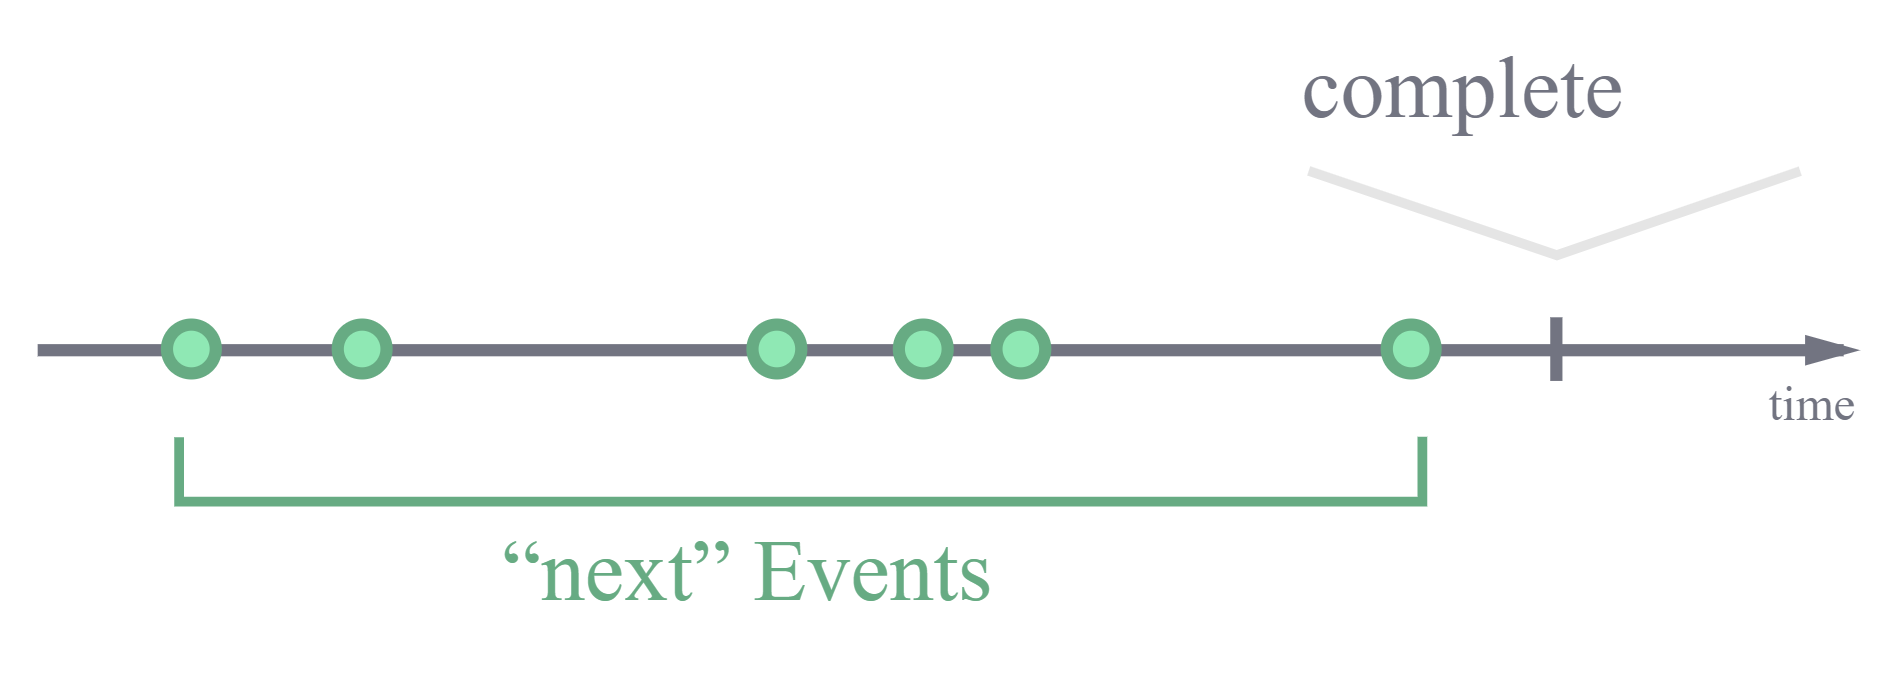
\includegraphics[width=0.5\textwidth]{images/cycle-streams.png}}}$
    \caption[]{Zasada działania strumieni \cite{bib:cycle-streams}}
    \label{fig:cycle-streams}
\end{figure}

Abstrakcja frameworku wydziela funkcję \texttt{main}, której argumentami są efekty odczytów ze świata zewnętrznego (\textit{sources}), a wyjściem są efekty zapisów w celu wpłynięcia na świat zewnętrzny (\textit{sinks}). Efekty I/O są zarządzane przez sterowniki (\textit{drivers}), a więc wtyczki obsługujące efekty DOM, zapytania HTTP, itp.

\begin{figure}[H]
	\centering
	$\vcenter{\hbox{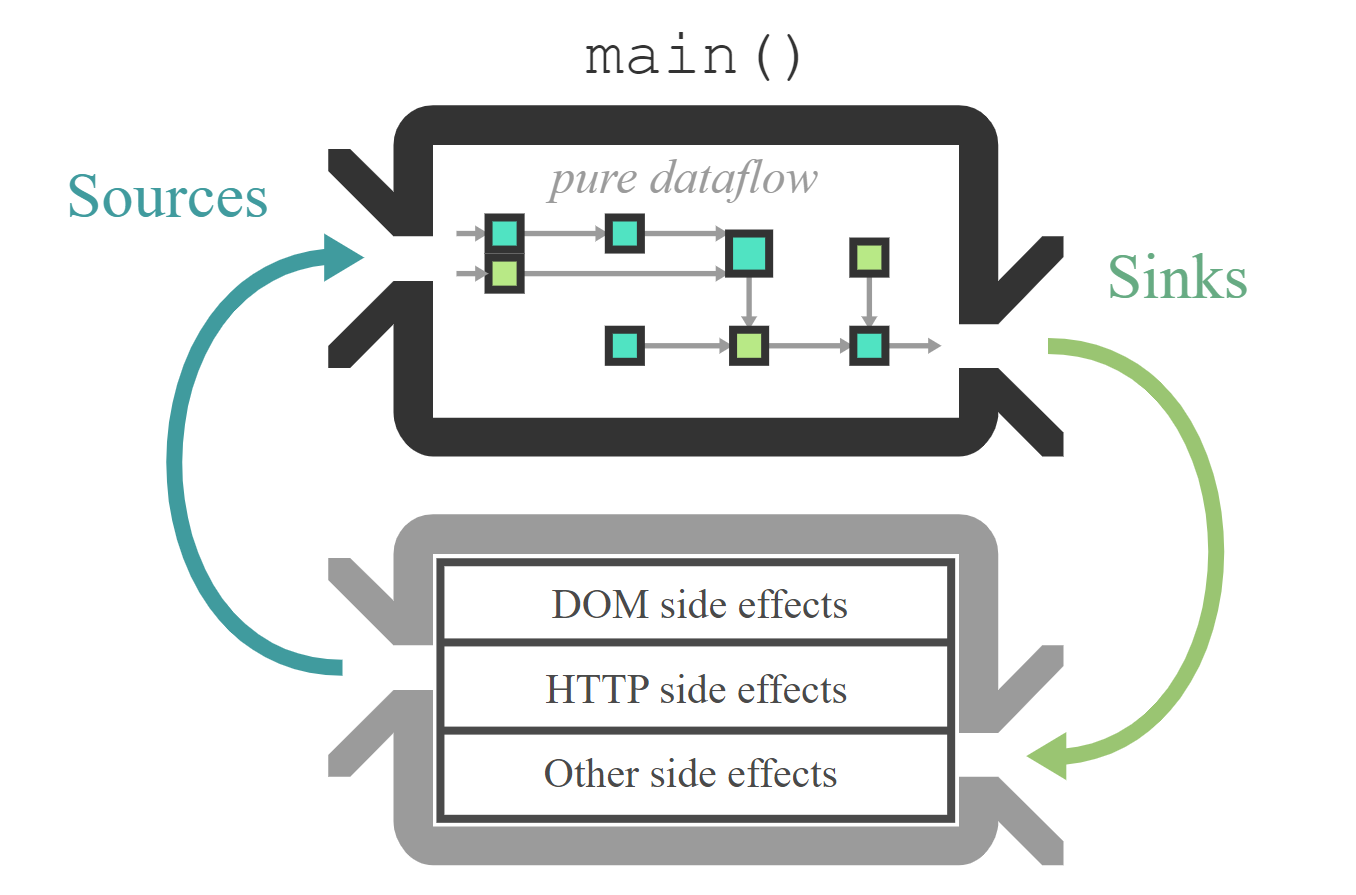
\includegraphics[width=0.5\textwidth]{images/cycle-dataflow.png}}}$
    \caption[]{Schemat przepływu danych w aplikacji Cycle.js \cite{bib:cycle-dataflow}}
    \label{fig:cycle-dataflow}
\end{figure}

Cycle.js wykorzystuje architekturę \textit{Model-View-Intent}. Architektura ta spełnia główne założenia \textit{Model-View-Controller}, jest reaktywna i funkcyjna. Reaktywność jest spowodowana tym, że \textit{Intent} obserwuje użytkownika (akcje wywołane z komputera), \textit{Model} obserwuje \textit{Intent}, \textit{View} obserwuje \textit{Model} oraz użytkownik obserwuje \textit{Intent}. Funkcyjność jest wynikiem tego, iż każdy z komponentów jest wyrażony poprzez funkcje na strumieniach.

\begin{figure}[H]
	\centering
	$\vcenter{\hbox{
\includegraphics[width=\textwidth]{images/cycle-mvi.png}}}$
    \caption[]{Dekompozycja funkcji \texttt{main} na \texttt{intent}, \texttt{model}, \texttt{view} \cite{bib:cycle-mvi}}
    \label{fig:cycle-mvi}
\end{figure}

\textit{Model-View-Intent} nie narzuca dekompozycji funkcji \texttt{main}, a więc podział na \textit{Model}, \textit{View} oraz \textit{Intent} nie jest konieczny. Jest to jednak wydajny sposób na organizację kodu i wydzielenie poszczególnych odpowiedzialności.

Cycle.js jest bardzo lekką biblioteką z dużymi możliwościami, dzięki czemu udostępnia programistom zestaw funkcji do tworzenia własnych sterowników i dostosowywania ich pod własne potrzeby. Widoki są generowane poprzez stworzenie \textit{virtual tree} za pomocą tagów \texttt{virtual-hyperscript}.


\chapter{Struktura i architektura aplikacji}
\section{Struktura aplikacji}
Katalogiem głównym aplikacji jest \texttt{app}. Znajdują się w nim różnorakie pliki konfiguracyjne - projektowe, bazodanowe, czy dotyczące edytora kodu. Znajdują się w nim również dwa katalogi: katalog \texttt{public} zawierający plik \texttt{index.html} specyfikujący tag \texttt{<div id='app'></div>}, wykorzystywany przez Vue w celu wyrenderowania aplikacji, jak i katalog \texttt{src} zawierający wszystkie pliki źródłowe. Znajdują się w nim katalogi:
\begin{itemize}
    \item \texttt{api} --- katalog zawierający implementację funkcji dotyczących zapytań CRUD do bazy danych wykorzystywanych przez komponenty,
    \item \texttt{assets} --- katalog zawierający style CSS,
    \item \texttt{components} --- katalog zawierający komponenty paska nawigacyjnego (\textit{navbar}) oraz stopki,
    \item \texttt{configs} --- katalog zawierający plik konfiguracyjny Firebase oraz wrapper wykorzystujący konfigurację w celu uzyskania obiektu bazy danych,
    \item \texttt{router} --- katalog z plikiem \texttt{vue-router} obsługujący przekierowania,
    \item \texttt{store} --- katalog z plikiem \texttt{vuex} przechowujący globalny stan aplikacji,
    \item \texttt{services} --- katalog zawierający komponenty Cycle.js, generatory obiektów, typy, funkcje pomocnicze,
    \item \texttt{tests} --- katalog zawierający testy jednostkowe
    \item \texttt{views} --- katalog zawierający komponenty Vue.js
\end{itemize}

\section{Zastosowana architektura}
Aplikacja CStrikers wykorzystuje dwa frameworki front-endowe: Vue.js oraz Cycle.js. Oznacza to, że wykorzystywane są architektury \textit{MVVM} oraz \textit{MVI}, opisane w poprzednim rozdziale. Bazą danych jest Firestore Database, udostępnione funkcje są używane w celu zaimplementowania wspólnego, reużywalnego API dla wszystkich komponentów.

Plik \texttt{main.js} odpowiada za inicializajcę aplikacji, wraz z użyciem \texttt{Vuex} służącego do przechowywania globalnego stanu we Vue, oraz z \texttt{vue-router} służącego do obsługi przekierowań.

Bazowym komponentem wykorzystanym przez aplikację jest \texttt{App.vue} - udostępnia on style oraz ogólny widok aplikacji (\textit{wrapper}). Pozostałe komponenty zaimplementowane we Vue korzystają z SFC i są wydzielone do osobnych plików w katalogu \texttt{views}. W celu zachowania spójności aplikacji, komponenty Cycle.js są wstrzykiwane do Vue poprzez handlery, które wywołują funkcję \texttt{run(main, drivers)}. W ten sposób uzyskano jednolity layout.

\begin{figure}[H]
	\centering
	$\vcenter{\hbox{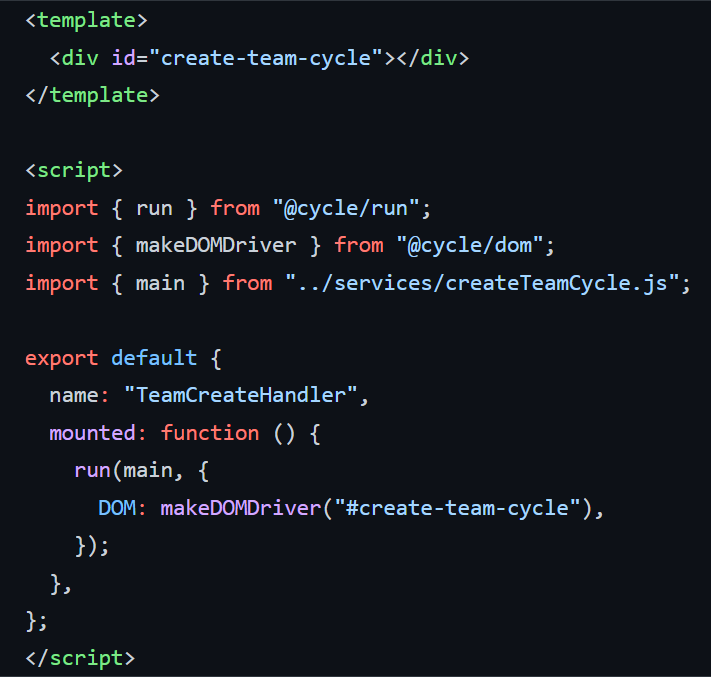
\includegraphics[width=0.9\textwidth]{images/vue-cycle-injection.png}}}$
    \caption[]{Przykład implementacji wstrzykiwania kodu Cycle.js do Vue.js}
    \label{fig:cycle-mvi}
\end{figure}

\chapter{Aplikacja}
\section{Cele aplikacji}

\begin{itemize}
    \item Tworzenie kont użytkowników oraz możliwość logowania się.
    \item Tworzenie drużyn przez istniejących użytkowników.
    \item Przegląd informacji o drużynach, ich członkach oraz turniejach w jakich brały udział.
    \item Możliwość tworzenia turniejów CSGO w różnych systemach.
    \item Możliwość ukrycia turnieju z listy wszystkich turniejów.
    \item Odrzucanie i wybieranie map przez kapitanów drużyn biorących udział w meczu odbywające się \textit{real-time}.
    \item Możliwość zapisania wyniku spotkania.
    \item Śledzenie postępów turnieju na podstawie listy wyników oraz tabeli.
\end{itemize}

\section{Opisy kolekcji Firestore Database}
Firestore Database jest bazą danych mającą podobną strukturę do MongoDB.

\subsection{Users}
Kolekcja korzystająca z kolekcji Users wbudowanej w Firebase Authentication. Przechowuje informacje o użytkownikach: ich pseudonim, imię i nazwisko, email oraz pole uid będące referencją.

\subsection{Teams}
Kolekcja zawierająca informacje o stworzonych drużynach. Polami dokumentów są: nazwa drużyny, ID użytkownika z kolekcji users będącego kapitanem drużyny oraz tablicę ID członków drużyny.

\subsection{Maps}
Kolekcja zawierająca mapy, na których rozgrywane są mecze.

\subsection{Matches}
Kolekcja przechowująca dokumenty dotyczące meczów. Zawiera pola będące ID obu drużyn, typ meczu, tablicę z wybranymi mapami, tablicę z odrzuconymi mapami, tablicę wyników każdej z wybranej map, liczbę wygranych map przez obie drużyny oraz nazwę drużyny, która wygrała.

\subsection{Tournaments}
Kolekcja przechowująca dokumenty dotyczące turniejów. Zawiera pola będące ID organizatora, informacje o widoczności turnieju, system w jakim rozgrywany jest turniej, typ rozgrywanych meczów (B01/BO3/BO5), tablicę ID drużyn biorących udział w turnieju, tablicę ID meczów rozgrywanych w ramach turnieju oraz nazwę drużyny, która wygrała turniej.

\section{Model obiektowy} % TODO
...

\section{Historyjki użytkownika}

\subsection{Gracz}
\textbf{Gracz} --- osoba chcąca rozgrywać mecze w turnieju.
\begin{itemize}
    \item Jako gracz, chcę zarejestrować się w aplikacji, żeby inny gracz mógł mnie dodać do swojej drużyny.
    \item Jako gracz, chcę stworzyć drużynę, żeby móc wziąć udział w turnieju.
    \item Jako gracz, chcę mieć możliwość łatwego odrzucania i wybierania map w meczach, w których biorę udział, żeby móc grać na mapach, które preferuje mój zespół.
    \item Jako gracz, chcę mieć możliwość wpisywania wyników spotkań, które rozgrywam, żeby wiedzieć w którym miejscu w tabeli/w której rundzie jest moja drużyna.
\end{itemize}

\subsection{Organizator turnieju}
\textbf{Organizator turnieju} --- użytkownik aplikacji chcący stworzyć turniej.

\begin{itemize}
    \item Jako organizator turnieju, chcę mieć możliwość wyboru drużyn, które wezmą udział w moim turnieju, żeby mieć pewność, że żadna niezaproszona drużyna nie weźmie w nim udziału.
    \item Jako organizator turnieju, chcę mieć możliwość ukrycia turnieju, żeby rozgrywki były prywatne.
    \item Jako organizator turnieju, chcę mieć możliwość wyboru typu rozgrywanych meczów, żeby kontrolować czas trwania i balans drużyn w turnieju.
    \item Jako organizator turnieju, chcę mieć możliwość wyboru systemu, w którym będzie rozgrywany turniej, żebym mógł spełnić swoje wymagania.
    \item Jako organizator turnieju, chcę mieć podgląd statystyk wszystkich rozgrywanych meczów, żeby kontrolować ich stan.
    \item Jako organizator turnieju, chcę wiedzieć kim jest zwycięzca turnieju, aby nie musieć przeglądać wszystkich spotkań i liczyć wyników manualnie.
\end{itemize}


\chapter{Implementacja aplikacji i jej przebieg}
Implementacja od początku sprawiała problemy, jednak po czasie udało się je rozwiązać i ukończyć aplikację zgodnie z założeniami.

Pierwszym pomysłem było stworzenie aplikacji opartej o Express.js oraz backendzie w JavaScript, jednak konfiguracja Vue.js oraz Cycle.js działających jednocześnie była bardzo kłopotliwa, gdyż na tamten moment część paczek była niekompatybilna. Podjąłem wtedy decyzję o zmianie Express.js na Pythona oraz Django, z wykorzystaniem Django Templates. Pomimo ukończonego wcześniej projektu w Pythonie, moja znajomość języka była zbyt niska, aby napisać łatwo rozszerzalny kod, więc po zaimplementowaniu dwóch komponentów kod był praktycznie nierozszerzalny, na co w dużej mierze wpływała ilość zagnieżdżeń oraz wzajemnych referencji encji.

Ostatnim rozwiązaniem, było napisanie aplikacji we Vue.js oraz Cycle.js, wykorzystując przy tym bazę danych Firestore Database. To pozwoliło na stworzenie API wykorzystywanego przez oba frameworki, dzięki czemu implementacja nie sprawiała aż tak dużych problemów. Największą trudność stanowiło jednak zaplanowanie struktur kolekcji, ich referencji oraz kroków implementacyjnych. Przez brak organizacji i konkretnego planu działania, musiałem wielokrotnie zmieniać kod i rozszerzać kolekcje, aby były kompatybilne ze wszystkimi działaniami, jakie można było podjąć w aplikacji.

Testowanie aplikacji ograniczone zostało do funkcji, które nie należały do bibliotek udostępniających m.in. obsługę baz danych, czy tworzenia V-DOM we Vue czy Cycle.js gdyż ich implementacje są w pełni przetestowane.

Dokumentacja aplikacji była sporządzana na bieżąco, w trakcie programowania - plusem takiego podejścia jest możliwość odnoszenia się do różnych funkcji bez konieczności analizowania ich działania, jednak przy częstych zmianach kodu wymagało to dodatkowego czasu.

\chapter{Podsumowanie}
Pierwszym krokiem w implementacji powinno być zaplanowanie struktury aplikacji, przygotowanie kolekcji obejmujących wszystkie możliwe rozwiązania oraz konfiguracja środowiska. Pominięcie któregoś z tych punktów może sprawić, że pisanie kodu będzie bardzo trudne, a potencjalne modyfikacje w przyszłości - niemożliwe. Bardzo ważne jest również podejście \textit{Test-Driven Development} - dzięki temu udało się uniknąć niepotrzebnego debugowania, które przy częstych zmianach kodu bez wykorzystania TDD jest praktycznie nieodłączną częścią.

Programowanie z użyciem dwóch frameworków jest skomplikowane. Narzucając Vue.js jako główną bibliotekę w projekcie, trudno było sprawić, aby Cycle.js zaczął działać tak, jak powinien. Po kilkunastu różnych próbach udało się je jednak ze sobą połączyć poprzez wstrzyknięcie funkcji \texttt{run(main, drivers)} do handlera we Vue. Niestety nie można rozdzielić tych frameworków całkowicie - globalny stan z \texttt{vuex} przechowuje dane o zalogowanym użytkowniku, a \texttt{vue-router} obsługuje przekierowania, a więc konieczne było importowanie bibliotek spoza Cycle.js, aby komponenty spełniały swoje zadania.

Kolejnym problemem wynikającym z użycia dwóch frameworków jest konieczność ciągłego przestawiania swojego podejścia. Różni się nie tylko składnia, czy wykorzystywane biblioteki, ale też architektura. W przypadku Vue.js działanie opiera się na obiektach, ich przekazywanie oraz manipulacja nie są skomplikowane. Cycle.js działa w oparciu o MVI, a wszelkie zmiany są oparte na podejściu funkcyjnym i strumieniach.

W aplikacjach znacznie większych niż CStrikers łączenie różnych frameworków frontendowych nie jest najlepszym pomysłem. Istniejące frameworki mają bardzo szerokie zastosowanie, często rozszerzane przez dodatkowe, niewymagane biblioteki, dzięki czemu ograniczenie się do jednego nie przyczyni się do pogorszenia jakości aplikacji - wręcz przeciwnie, korzystając tylko z jednego frameworku programiście będzie znacznie łatwiej pisać kod zgodny z praktykami dobrego programowania oraz szybciej zyska biegłość, co znacząco przyspieszy implementację.


\chapter{Opis techniczny}
Aplikacja została napisana w języku Vue.js (wersja 3.0.0) oraz Cycle.js (\texttt{@cycle/dom} w wersji 23.1.0 oraz \texttt{@cycle/run} w wersji 5.7.0). Backend aplikacji obsługujący zapytania bazodanowe oraz logikę aplikacji został napisany w JavaScript. Testy jednostkowe zostały zaimplementowane przy użyciu Jest (wersja 28.1.1), a dokumentacja wygenerowana przez JSDoc (wersja 3.6.10). Za bazę danych posłużył Firestore Database dostarczany przez Firebase.

Kod aplikacji znajduje się w repozytorium GitHub:\newline
\url{https://github.com/whiskeyo/csgo-tournament}

\chapter{Polecenia aplikacji CStrikers}
Zestaw najważniejszych poleceń znajduje się w pliku \texttt{README.md}, są to m.in:
\begin{itemize}
    \item instalacja vue-cli: \texttt{sudo npm install -g @vue/cli}
    \item instalacja paczek NPM: \texttt{cd app; npm install}
    \item uruchomienie serwera developerskiego: \texttt{npm run dev}
    \item kompilacja projektu z możliwością hostowania na serwerach: \texttt{npm run build}
    \item uruchomienie lintera wskazującego błędy w kodzie: \texttt{npm run lint}
    \item uruchomienie formattera: \texttt{npm run format}
    \item uruchomienie testów jednostkowych: \texttt{npm run test}
    \item wygenerowanie pokrycia kodu: \texttt{npm run coverage}
    \item wygenerowanie dokumentacji: \texttt{npm run docs}
\end{itemize}


%%%%% BIBLIOGRAFIA

\begin{thebibliography}{1}
    \bibitem{bib:vue-sfc} Vue.js - Introduction, Single-File Components - \url{https://vuejs.org/guide}
    \bibitem{bib:vue-lifecycle-hooks} Vue.js - Lifecycle Diagram - \url{https://vuejs.org/guide/essentials/lifecycle.html#lifecycle-diagram}
    \bibitem{bib:vue-router-getting-started} Vue Router - Getting Started - \url{https://router.vuejs.org/guide/}
    \bibitem{bib:vuex-getting-started} Vuex - Getting Started - \url{https://vuex.vuejs.org/guide/}
    \bibitem{bib:cycle-streams} Cycle.js - Streams - \url{https://cycle.js.org/streams.html}
    \bibitem{bib:cycle-dataflow} Cycle.js - Dataflow - \url{https://cycle.js.org/#-dataflow}
    \bibitem{bib:cycle-mvi} Cycle.js - Model-View-Intent - \url{https://cycle.js.org/model-view-intent.html}
    \bibitem{bib:cycle-getting-started} Cycle.js - Getting started - \url{https://cycle.js.org/getting-started.html}
    \bibitem{bib:cycle-api-reference} Cycle.js - API reference - \url{https://cycle.js.org/api/index.html#api-reference}
    \bibitem{bib:firestore-docs} Firestore Database - Documentation - \url{https://firebase.google.com/docs/firestore}
\end{thebibliography}

\end{document}
